%%%%%%%% STAT 453 MIDWAY REPORT (ICML 2026 TEMPLATE) %%%%%%%%%%%%%%%%%%%%%%%%%%%%%%
% Build:  latexmk -pdf midway_report.tex      (figures: python make_figures.py)
% All numbers come from ../results/ (written by scripts/evaluate.py).

\documentclass{article}

\usepackage{microtype}
\usepackage{graphicx}
\usepackage{booktabs}
\usepackage{hyperref}
\newcommand{\theHalgorithm}{\arabic{algorithm}}

% [preprint] shows the author names (the default blind mode hides them) and,
% unlike [accepted], does not print an ICML proceedings notice. The notice
% line at the end of the first-page footnote (where published papers say
% "Proceedings of ICML ...") is replaced with the course name.
\usepackage[preprint]{icml2026}
\makeatletter
\renewcommand{\ICML@preprint}{\textit{STAT 453 Midway Report, November 2026.}}
\makeatother

\usepackage{amsmath}
\usepackage{amssymb}
\usepackage[capitalize,noabbrev]{cleveref}

\icmltitlerunning{Comparing VAEs and GANs for Unsupervised Tumor Detection in Brain MRI}

\begin{document}

\twocolumn[
  \icmltitle{Learning Healthy Anatomy to Find Tumors: Comparing VAEs and GANs\\
    for Unsupervised Anomaly Detection in Brain MRI (Midway Report)}

  \icmlsetsymbol{equal}{*}  % "*" after each name = equal contribution

  \begin{icmlauthorlist}
    \icmlauthor{Jenny Brant}{equal,uw}
    \icmlauthor{Abhijeet Beedikar}{equal,uw}
    \icmlauthor{Diya Kothari}{equal,uw}
    \icmlauthor{Daksh Kacham}{equal,uw}
  \end{icmlauthorlist}

  % These fill the first-page footnote: "1Department of ... Correspondence to: ..."
  \icmlaffiliation{uw}{Department of Statistics, University of Wisconsin--Madison, Madison, WI, USA}
  \icmlcorrespondingauthor{Jenny Brant}{jobrant@wisc.edu}
  \icmlcorrespondingauthor{Abhijeet Beedikar}{beedikar@wisc.edu}
  \icmlcorrespondingauthor{Diya Kothari}{ddkothari@wisc.edu}
  \icmlcorrespondingauthor{Daksh Kacham}{kacham@wisc.edu}

  \icmlkeywords{Anomaly detection, VAE, GAN, brain MRI}
  \vskip 0.3in
]

\printAffiliationsAndNotice{\icmlEqualContribution}

\begin{abstract}
Supervised tumor segmentation needs thousands of expert-drawn outlines and only
recognizes the diseases it was trained on. We instead train generative models
only on \emph{healthy} brain MRI and flag the regions a model cannot
reconstruct. We compare a variational autoencoder (VAE), f-AnoGAN (a Wasserstein
GAN with an encoder) and a plain autoencoder (AE) under one shared pipeline.
Models are trained on 462 healthy IXI subjects (T2) and tested on 436 glioma
patients from the Medical Segmentation Decathlon. So far we have built the full
pipeline, including our own PyTorch affine registration, and evaluated all three
models at $64\times64$. In preliminary single-seed runs the VAE is best (subject
Dice $0.51$, pixel AUROC $0.89$), f-AnoGAN
is close (Dice $0.47$) with the fewest complete misses, and the plain AE does not
beat a simple ``bright on T2'' intensity baseline on Dice ($0.38$ vs.\ $0.39$).
Our main challenges were registration failures and CPU-only training. Next we will move to the proposal's $128\times128$ resolution, add
seeds and confidence intervals, and sweep the VAE's KL weight and latent size.
\end{abstract}

%=============================================================================
\section{Introduction}
%=============================================================================

Most deep learning tools for medical imaging are supervised: they learn from
scans in which a radiologist has outlined every lesion. Such labels are slow and
expensive to produce, and a supervised model only recognizes the abnormalities
it was shown. Healthy scans, by contrast, are plentiful.

We ask whether a generative model that has only ever seen healthy brains can
detect and localize brain tumors, and whether a VAE or a GAN does this better.
The idea is to learn the distribution of healthy anatomy, $p(\mathbf{x})$. When
the model is shown a scan with a tumor, it ``repairs'' the image toward the
nearest healthy-looking brain $\hat{\mathbf{x}}$, and the residual
$\mathbf{x}-\hat{\mathbf{x}}$ highlights what does not belong. Because no tumor
labels are used for training, this \emph{unsupervised anomaly detection} could
flag abnormalities nobody trained it to find.

Generative models are central to this approach. A plain autoencoder only learns
to copy its input, and with enough capacity it copies tumors too. A VAE (latent
prior) and a GAN (realism critic) both restrict reconstructions to images that
look like the training distribution. VAEs are stable but blurry, so fine edges
cause false alarms. GANs are sharp but harder to train and may not cover all of
healthy anatomy. Published comparisons disagree, partly because they use different
private data and preprocessing~\cite{baur2021comparative}. Our contribution is a
controlled comparison on public data, with identical preprocessing and
post-processing for every model.

%=============================================================================
\section{Related Work}
%=============================================================================

\textbf{Generative models.} VAEs~\cite{kingma2014vae} maximize a lower bound on
the data likelihood with an encoder--decoder pair and a Gaussian latent prior.
GANs~\cite{goodfellow2014gan} train a generator against a discriminator;
DCGAN~\cite{radford2016dcgan} and WGAN-GP~\cite{gulrajani2017wgangp} made this
stable on images. We use DCGAN-style layers for all models so that differences
come from the training objective, not the architecture.

\textbf{GANs for anomaly detection.} AnoGAN~\cite{schlegl2017anogan} was the first
to use a GAN trained on healthy images to localize anomalies in medical images.
It finds the closest healthy image by optimizing the latent code separately for
every test image, which is slow. f-AnoGAN~\cite{schlegl2019fanogan} replaces this
search with an encoder trained after the WGAN-GP, giving a single forward pass.
We adopt f-AnoGAN as our GAN representative.

\textbf{Autoencoders on brain MRI.} \citet{baur2018deep} combined a VAE with an
adversarial loss to segment multiple-sclerosis lesions without labels.
\citet{chen2018constrained} constrained the latent space of an adversarial
autoencoder for brain lesions, and \citet{zimmerer2019localization} showed that
VAE gradients and the KL term also carry localization information. The
comparative study of \citet{baur2021comparative} benchmarked many AE and GAN
variants on shared data. It found that results depend heavily on preprocessing
and post-processing, and that no model family clearly wins.
\citet{meissen2021challenging} went further: on FLAIR scans a simple intensity
threshold matched or beat these deep models, because tumors are simply
hyperintense. More recent work uses diffusion models~\cite{pinaya2022diffusion},
but VAEs and GANs remain the standard reference points.

\textbf{Our position.} We therefore use only public data~\cite{ixi,antonelli2022msd,menze2015brats},
share all preprocessing and scoring between models, and add a plain AE and the
intensity baseline of \citet{meissen2021challenging} as controls.

%=============================================================================
\section{Methods (Implemented)}
%=============================================================================

\subsection{Preprocessing pipeline}
\label{sec:preproc}

IXI and MSD come from different scanners and were processed differently, so a
model could flag ``different hospital'' instead of ``tumor''. We therefore apply
one pipeline to every scan:
(1)~reorient to RAS and roughly rescale intensities;
(2)~affinely register (12 parameters) to the MNI152 2009a template~\cite{fonov2011mni};
(3)~skull-strip with the template's brain mask (MSD scans are already
skull-stripped, so we also intersect with their own brain outline);
(4)~divide by the 99th percentile of brain intensities and clip to $[0,1]$;
(5)~keep axial slices whose brain area is at least 30\% of the maximum, taking
every second level, crop around the brain and resize to $128\times128$ by area
averaging. The $64\times64$ inputs are pooled from these slices.

\textbf{Challenge 1: no registration library.} Our team develops on Windows
laptops with ARM processors (Snapdragon X Elite). SimpleITK, ANTs and dipy have
no builds for this platform, and neither does any dedicated skull-stripping
tool. We therefore wrote affine registration ourselves in PyTorch. It resamples
with \texttt{grid\_sample}, maximizes normalized cross-correlation (NCC) with
Adam, works coarse to fine (4\,mm, then 2\,mm), and uses a random subset of
40k voxels per step for speed. A unit test confirms it recovers a known affine
transform to under 1\,mm. Nilearn ships only a T1 template, so we built a
T2-like template from its gray- and white-matter probability maps
(CSF $=1.0$, GM $=0.55$, WM $=0.35$, matching T2 contrast).

\textbf{Challenge 2: registration failures.} In our first full run, about 30\%
of IXI scans registered badly (NCC $\approx 0$, with the eyes inside the brain
mask). Head tilt and a poor centre-of-mass start trapped the optimizer in local
minima. What worked was a coarse 6\,mm grid search over pitch ($\pm 25^\circ$),
shifts ($\pm 20$/$\pm 40$\,mm) and scale ($0.8$--$1.0$), refining the three best
starts. All 578 IXI and 484 MSD scans then pass a visual check (median NCC
$0.47$ and $0.25$); the lowest MSD scores are well-aligned scans with very large
tumors.

\subsection{Models}

All models share DCGAN-style networks. The encoder applies four stride-2
$4\times4$ convolutions ($1{\to}32{\to}64{\to}128{\to}256$ channels,
LeakyReLU 0.2, batch norm), turning a $64\times64$ image into a $256\times4\times4$
feature map, followed by a linear layer. The decoder mirrors this with
transposed convolutions and a sigmoid output. The latent size is $d=128$, and
weights follow the DCGAN initialization.

\textbf{AE} (2.44M parameters) minimizes
$\|\mathbf{x}-D(E(\mathbf{x}))\|_2^2$.

\textbf{VAE} (2.96M) minimizes the negative ELBO with a Gaussian decoder:
\begin{equation}
\mathcal{L}_{\text{VAE}} = \|\mathbf{x}-D(\mathbf{z})\|_2^2
 + \beta\,\mathrm{KL}\big(q(\mathbf{z}|\mathbf{x})\,\|\,\mathcal{N}(\mathbf{0},I)\big),
\end{equation}
with $\mathbf{z}=\boldsymbol\mu+\boldsymbol\sigma\odot\boldsymbol\epsilon$
(the reparameterization trick) and $\beta=1$. At test time we decode the
posterior mean.

\textbf{f-AnoGAN} (3.13M) is trained in two stages. Stage~1 is a WGAN-GP: the
generator $G$ is the decoder architecture and the critic $C$ is the encoder
architecture with layer normalization instead of batch normalization, because
the gradient penalty is computed per sample. The critic minimizes
$\mathbb{E}[C(G(\mathbf{z}))]-\mathbb{E}[C(\mathbf{x})]
+\lambda\,\mathbb{E}[(\|\nabla_{\tilde{\mathbf{x}}}C(\tilde{\mathbf{x}})\|_2-1)^2]$
with $\lambda=10$ and $n_{\text{critic}}=5$. Stage~2 freezes $G$ and $C$ and
trains an encoder $E$ with the izi$_f$ loss
$\|\mathbf{x}-G(E(\mathbf{x}))\|^2+\kappa\|f(\mathbf{x})-f(G(E(\mathbf{x})))\|^2$,
where $f$ denotes the critic's last feature map and $\kappa=1$.

\subsection{Anomaly scoring}

Following (A3), our main anomaly map keeps only the \emph{positive} residual:
\begin{equation}
A = \big(g_{\sigma} * \max(\mathbf{x}-\hat{\mathbf{x}},\,0)\big)\odot M_{\ominus},
\end{equation}
where $g_\sigma$ is a Gaussian ($\sigma=1$ pixel) and $M_\ominus$ is the brain
mask eroded by 2 pixels, because reconstructions are least reliable at the brain
border. A pixel is labelled tumor if $A>\tau$. The threshold $\tau$ maximizes
Dice on a held-out MSD validation set. A slice's score is the mean of its top
1\% of anomaly values. We also report the plain absolute residual
$|\mathbf{x}-\hat{\mathbf{x}}|$ as an ablation. The \emph{intensity baseline}
uses $\hat{\mathbf{x}}=\mathbf{0}$, so it detects ``bright = tumor''.

\subsection{Assumptions}
\label{sec:assumptions}

We state the method's assumptions explicitly, since each can fail.
\textbf{(A1) Healthy training data:} every IXI scan is free of pathology (IXI
volunteers were not screened for incidental findings).
\textbf{(A2) Anomalies are not reconstructed:} a model trained only on healthy
anatomy maps a tumor to healthy tissue. This requires that it cannot simply
copy its input; the AE shows this can fail (\cref{sec:results}).
\textbf{(A3) Tumors are bright on T2:} edema and most tumor tissue are
hyperintense, so we score only $\mathbf{x}-\hat{\mathbf{x}}>0$; dark parts such
as necrotic cores are missed.
\textbf{(A4) Comparable inputs:} after affine registration, one shared template
mask and 99th-percentile scaling, the residual reflects pathology rather than
scanner or site differences between IXI and MSD. Affine alignment does not match
individual folds, and the mask is approximate at the brain border.
\textbf{(A5) Independent 2D slices:} slices are scored without 3D context, and
left--right flips assume healthy brains are roughly symmetric.
\textbf{(A6) Labels only for the threshold:} the merged whole-tumor mask is the
reference, and one global $\tau$, chosen on 48 labelled MSD subjects assumed to
match the test distribution, is used for all subjects.
\textbf{(A7) VAE likelihood:} the summed squared error corresponds to a Gaussian
decoder with the same fixed variance for every pixel.

\textbf{Challenge 3: compute.} All results so far were run without a GPU, on a
Windows laptop with an ARM processor. The x64 PyTorch build under emulation
(oneDNN kernels) trained 2.6$\times$ faster than the native ARM64 build (670 vs.\
257 images/s), so we use it, with the three models in parallel. This limit is why
we use the proposal's $64\times64$ ``fast experiment'' setting.

%=============================================================================
\section{Experiments}
%=============================================================================

\begin{table*}[t]
\caption{Test results at $64\times64$ (positive residual). Dice is computed per
subject (mean $\pm$ sd over 436 MSD test subjects) and over all test pixels
pooled (global). Slice AUROC (MSD) separates tumor slices from tumor-free slices
of MSD patients. Slice AUROC (vs.\ IXI) separates MSD tumor slices from healthy
IXI test slices. FPR is the fraction of healthy IXI test brain pixels flagged at
the chosen threshold. Best value per column in bold.}
\label{tab:main}
\vskip 0.05in
\centering
\small
\begin{tabular}{lccccccc}
\toprule
 & Dice & Dice & Pixel & Pixel & Slice AUROC & Slice AUROC & Healthy \\
Model & (subject) & (global) & AUROC & AUPRC & (MSD) & (vs.\ IXI) & FPR \\
\midrule
Intensity baseline & $0.394 \pm 0.243$ & 0.431 & 0.854 & 0.351 & 0.779 & 0.772 & 4.52\% \\
AE                 & $0.380 \pm 0.161$ & 0.420 & 0.796 & 0.402 & \textbf{0.869} & 0.865 & 4.01\% \\
VAE                & $\mathbf{0.514 \pm 0.227}$ & \textbf{0.566} & \textbf{0.894} & \textbf{0.575} & 0.867 & 0.929 & \textbf{1.21\%} \\
f-AnoGAN           & $0.474 \pm 0.183$ & 0.517 & 0.855 & 0.514 & 0.867 & \textbf{0.931} & 1.31\% \\
\bottomrule
\end{tabular}
\end{table*}

\begin{figure*}[t]
\centering
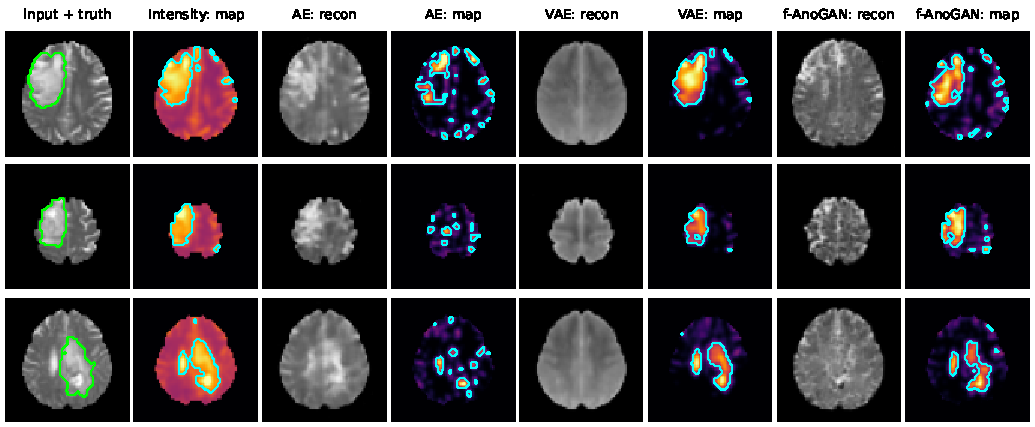
\includegraphics[width=\textwidth]{figures/examples.pdf}
\caption{MSD test slices (rows) with each model's healthy reconstruction and
anomaly map. Green: expert whole-tumor outline. Cyan: predicted tumor at the
threshold chosen on validation. The VAE's blurry reconstruction leaves one
compact anomaly. f-AnoGAN is sharper but adds scattered false positives where
folds are misplaced. The AE partly reconstructs the tumor itself, which weakens
its map.}
\label{fig:examples}
\end{figure*}

\subsection{Data and setup}

\textbf{Training data:} IXI~\cite{ixi}, 578 healthy adults, T2-weighted, split
80/10/10 by subject into 462 training, 58 validation and 58 test subjects
(26{,}796 training slices). \textbf{Test data:} MSD Task01
BrainTumour~\cite{antonelli2022msd}, 484 glioma patients from
BraTS~\cite{menze2015brats}. We use the T2 channel and merge all tumor labels
into one ``whole tumor'' mask. 48 subjects (10\%) are used only to choose the
threshold $\tau$, and 436 subjects (25{,}288 slices) are the test set. Tumor
pixels make up 9.2\% of MSD test brain pixels.
\textbf{Training:} Adam with learning rate $2{\cdot}10^{-4}$ and batch size 64,
random left--right flips, 40 epochs for AE and VAE. f-AnoGAN uses 60 WGAN-GP
epochs (learning rate $10^{-4}$, $\beta=(0,0.9)$) followed by 30 encoder epochs.
We keep the checkpoint with the lowest healthy validation MSE. Training took
2.9\,h for AE and VAE and 6.3\,h for f-AnoGAN on CPU.
\textbf{Metrics} follow the proposal: Dice, pixel AUROC and AUPRC, two slice
AUROCs, and the false-positive rate on healthy IXI test pixels.

\subsection{Preliminary results}
\label{sec:results}

\textbf{Training behaved as expected} (\cref{fig:curves}). The AE reaches by far
the lowest healthy reconstruction error ($2.1\cdot10^{-3}$, vs.\
$4.7\cdot10^{-3}$ for the VAE and $5.6\cdot10^{-3}$ for f-AnoGAN). The
Wasserstein estimate falls steadily from 35.5 to 1.5 without collapse.

\begin{figure}[t]
\centering
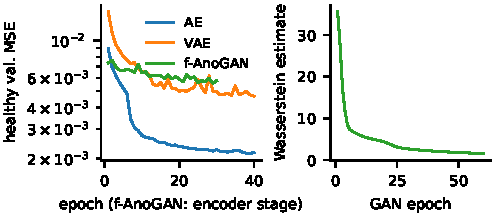
\includegraphics[width=\columnwidth]{figures/curves.pdf}
\caption{Left: reconstruction error on healthy IXI validation slices. Right:
the f-AnoGAN critic's Wasserstein estimate during GAN training.}
\label{fig:curves}
\end{figure}

\textbf{The VAE and f-AnoGAN outperform the AE and intensity baseline on
subject-level Dice in our preliminary experiments} (\cref{tab:main}). The VAE is
best on every pixel-level metric. It improves subject Dice by about $0.13$ over
the AE and $0.12$ over the intensity baseline, while reducing healthy-pixel
false positives by factors of 3.3 and 3.7, respectively. f-AnoGAN comes second on pixel metrics and
ties the VAE at slice level (AUROC $0.93$ vs.\ healthy IXI). The plain AE, despite
reconstructing healthy brains best, has the \emph{lowest} pixel AUROC
($0.80$). \Cref{fig:examples} shows why: it reconstructs part of the tumor too,
so the residual misses it, violating (A2): good reconstruction is not the goal;
reconstructing \emph{only} healthy anatomy is. The intensity baseline is strong at pixel level (AUROC $0.85$),
in line with \citet{meissen2021challenging}, but poor at slice level ($0.77$),
since many bright healthy structures such as ventricles and CSF also trigger it.

\textbf{Post-processing matters.} With the absolute residual instead of the
positive one, every model loses Dice (VAE $0.514\to0.484$, f-AnoGAN
$0.474\to0.435$, AE $0.380\to0.334$). The healthy FPR of f-AnoGAN doubles
($1.3\%\to2.6\%$), because dark mismatches at fine folds are now counted.

\textbf{Small tumors are the main failure mode} (\cref{fig:size}). Splitting
test subjects into thirds by tumor size, VAE Dice rises from $0.34$ (small) to
$0.65$ (large), and every model shows this pattern. The VAE leads on large
tumors ($0.65$ vs.\ $0.57$), but
f-AnoGAN has the fewest near-complete misses: 8.7\% of subjects have Dice $<0.2$,
compared with 11.7\% for the VAE, 14.7\% for the AE and 28.2\% for the baseline.
f-AnoGAN's scattered false positives thus mostly hurt on large tumors, where
Dice depends on boundary quality.

\begin{figure}[t]
\centering
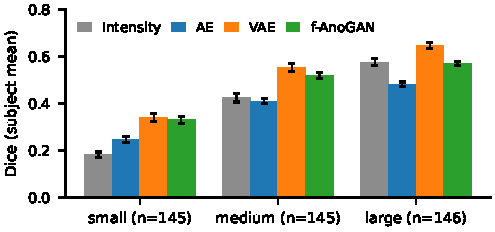
\includegraphics[width=\columnwidth]{figures/tumour_size.pdf}
\caption{Subject Dice by tumor-size tertile (whole-tumor pixels summed over a
subject's $64\times64$ slices). Error bars show the standard error.}
\label{fig:size}
\end{figure}

\textbf{Caveats.} Each number comes from a single training run (seed 42), so
differences of a few Dice points are not yet established. Assumption (A4) holds
only partly: template-mask skull stripping leaves a thin rim of skull on some IXI
scans, so part of every residual reflects domain shift.

%=============================================================================
\section{Conclusion and Updated Plan}
%=============================================================================

\textbf{Progress.} In our single-seed $64\times64$ runs, both generative models beat a
plain AE, the VAE is best on average and f-AnoGAN has the fewest near-complete
misses. \textbf{Changes from the proposal:}
our own registration and T2 template (no standard tool runs on our hardware),
plus the intensity baseline and positive-residual scoring
from~\citet{meissen2021challenging}.

\textbf{Next steps (by priority).}
(1)~\emph{Robustness:} 3 seeds per model, bootstrap confidence intervals over
subjects, and a paired Wilcoxon test of VAE vs.\ f-AnoGAN Dice.
(2)~\emph{Resolution:} train at $128\times128$, the proposal's main setting.
This needs about 4$\times$ more compute (over 24\,h for f-AnoGAN on the laptop
CPU), so we plan to migrate training to a Google Colab GPU runtime.
(3)~\emph{VAE trade-off:} sweep $\beta\in\{0.5,1,2\}$ and latent size
$d\in\{128,256\}$ to measure how blur trades sharpness against false alarms.
(4)~\emph{Error analysis:} results by tumor sub-region, and whether
HD-BET~\cite{isensee2019hdbet} skull stripping on Colab reduces border false
positives (testing A4).

\textbf{Timeline.}
\emph{Nov 9--20:} seed repeats and confidence intervals; migrate to a Colab GPU
runtime; start $128\times128$ runs. \emph{Nov 23:} $\beta$/latent sweep;
sub-region analysis. \emph{Nov 30:} HD-BET ablation; freeze experiments.
\emph{Dec 7:} final report.

\clearpage
\bibliography{references}
\bibliographystyle{icml2026}

\end{document}
